 
\chapter{Lasso}
 
\section{Introduction to the lasso}

Ridge regression works well for prediction, but it may be difficult
to interpret many small but non-zero coefficients. \citet{tibshirani1996regression} proposed to use the lasso, the acronym for the Least Absolute Shrinkage
and Selection Operator, to achieve the ambitious goal of simultaneously
estimating parameters and selecting important variables in the linear
regression. By changing the penalty term in the ridge regression,
the lasso automatically estimates some parameters as zero, dropping
them out of the model and thus selecting the remaining variables as
important predictors. 


\citet{tibshirani1996regression} defined the lasso as 
\begin{align}
\hat{\beta}^{\text{lasso}}(t) & =\arg\min_{b_{0},b_{1},\ldots,b_{p}}\textsc{rss}(b_0,b_1,\ldots,b_p)  \nonumber \\
 & \ \text{s.t. }\sum_{j=1}^{p}|b_{j}|\ensuremath{\leq t} .\label{eq:lasso-form2}
\end{align}
\citet{osborne2000lasso} studied its dual form
\begin{equation}
\hat{\beta}^{\text{lasso}}(\lambda)=\arg\min_{b_{0},b_{1},\ldots,b_{p}}\left\{\textsc{rss}(b_0,b_1,\ldots,b_p) +\lambda\sum_{j=1}^{p}|b_{j}|\right\} . \label{eq:lasso-form1}
\end{equation}
The two forms of lasso are equivalent in the sense that for a given $\lambda$ in \eqref{eq:lasso-form1}, there exists a $t$ such that the solution for \eqref{eq:lasso-form2} is identical to the solution for \eqref{eq:lasso-form1}. In particular, $t = \sum_{j=1}^p \hat{\beta}^{\text{lasso}}_j(\lambda) $. 
Technically, the minimizer of the lasso problem may not be unique especially when $p>n$, so the right-hand sides of the optimization problems should be a set. Fortunately, even though the minimizer may not be unique, the resulting predictor is always unique. \citet{tibshirani2013lasso} clarifies this issue.


Both forms of the lasso are useful. 
We will use the form (\ref{eq:lasso-form1}) for computation and use the form \eqref{eq:lasso-form2} for geometric intuition. Similar to the
ridge estimator, the lasso is not invariant to the linear transformation
of $X$. We proceed after standardizing the covariates and outcome as Condition \ref{condition::standardization}. For the same reason as the ridge, we can drop the intercept after standardization. 




\section{Comparing the lasso and ridge: a geometric perspective}


The ridge and lasso are very similar: both minimize a penalized version of the residual sum of squares. They differ in the penalty term: ridge uses an $L_2$ penalty, i.e., the $L_2$ norm of the coefficient $ \| b\|^2 =  \sum_{j=1}^p b_j^2$, and lasso uses an $L_1$ penalty, i.e., the $L_1$ norm of the coefficient   $\| b\|_1 = \sum_{j=1}^p | b_j |$. Compared to the ridge, the lasso can give sparse solutions due to the non-smooth penalty term. That is, estimators of some coefficients are exactly zero. 


Focus on the form \eqref{eq:lasso-form2}.  We can gain insights from the contour plot of the residual sum of squares as a function of $b$. With a well-defined OLS estimator $\hat{\beta}$, Theorem \ref{thm::geometryofols} ensures 
\begin{align*}
(Y-Xb)^{\T}(Y-Xb)  =(Y-X\hat{\beta})^{\T}(Y-X\hat{\beta})
  +(b-\hat{\beta})^{\T}X^{\T}X(b-\hat{\beta}),
\end{align*}
which equals a constant term plus a quadratic function centered at the OLS coefficient. Without any penalty, the minimizer is of course the OLS coefficient. With the $L_1$ penalty, the OLS coefficient may not be in the region defined by $\sum_{j=1}^{p}|b_{j}| \leq t$. If this happens, the intersection of the contour plot of $(Y-Xb)^{\T}(Y-Xb)$ and the border of the restriction region $\sum_{j=1}^{p}|b_{j}| \leq t$ can be at some axis. For example, Figure \ref{fig::lasso-sparse} shows a case with $p=2$, and the lasso estimator hits the x-axis, resulting in a zero coefficient for the second coordinate. However, this does not mean that lasso always generates sparse solutions because sometimes the intersection of the contour plot of $(Y-Xb)^{\T}(Y-Xb)$ and the border of the restriction region is at an edge of the region. For example, Figure \ref{fig::lasso-non-sparse} shows a case with a non-sparse lasso solution. 


\begin{figure}
\centering
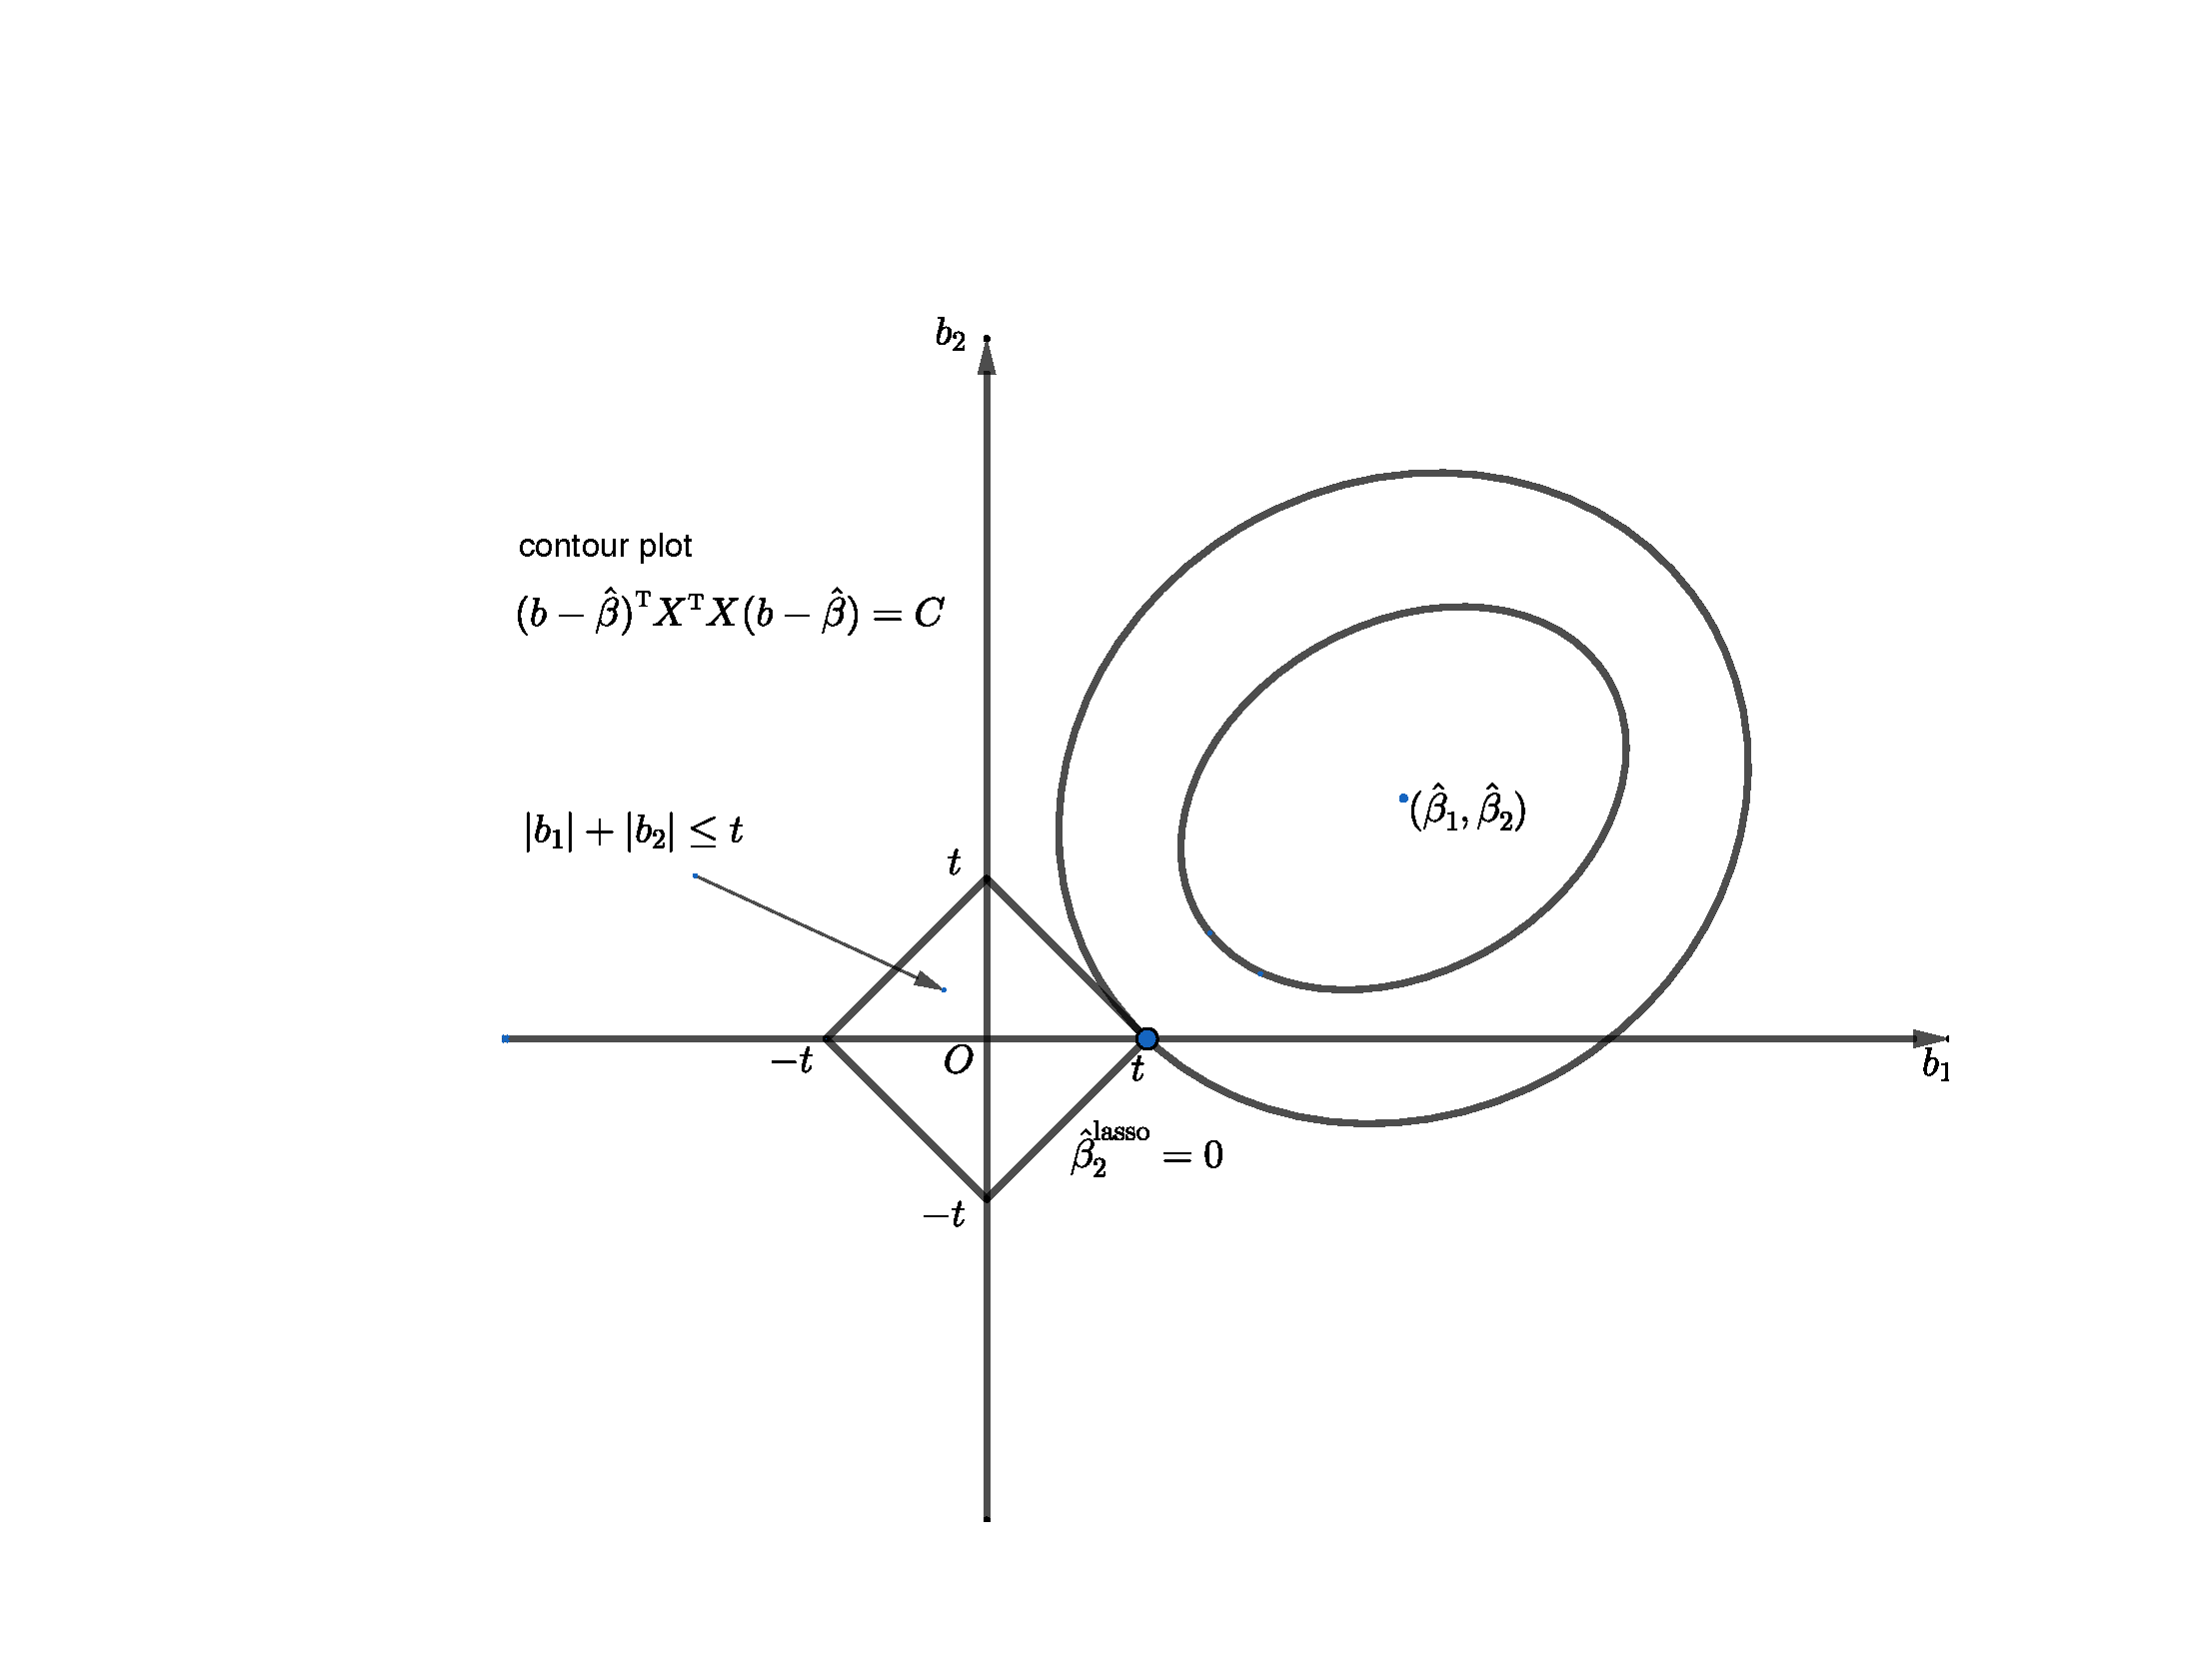
\includegraphics[width = 0.7\textwidth]{figures/lassogeometry1.pdf}
\caption{Lasso with a sparse solution}\label{fig::lasso-sparse}
\end{figure}

\begin{figure}
\centering 
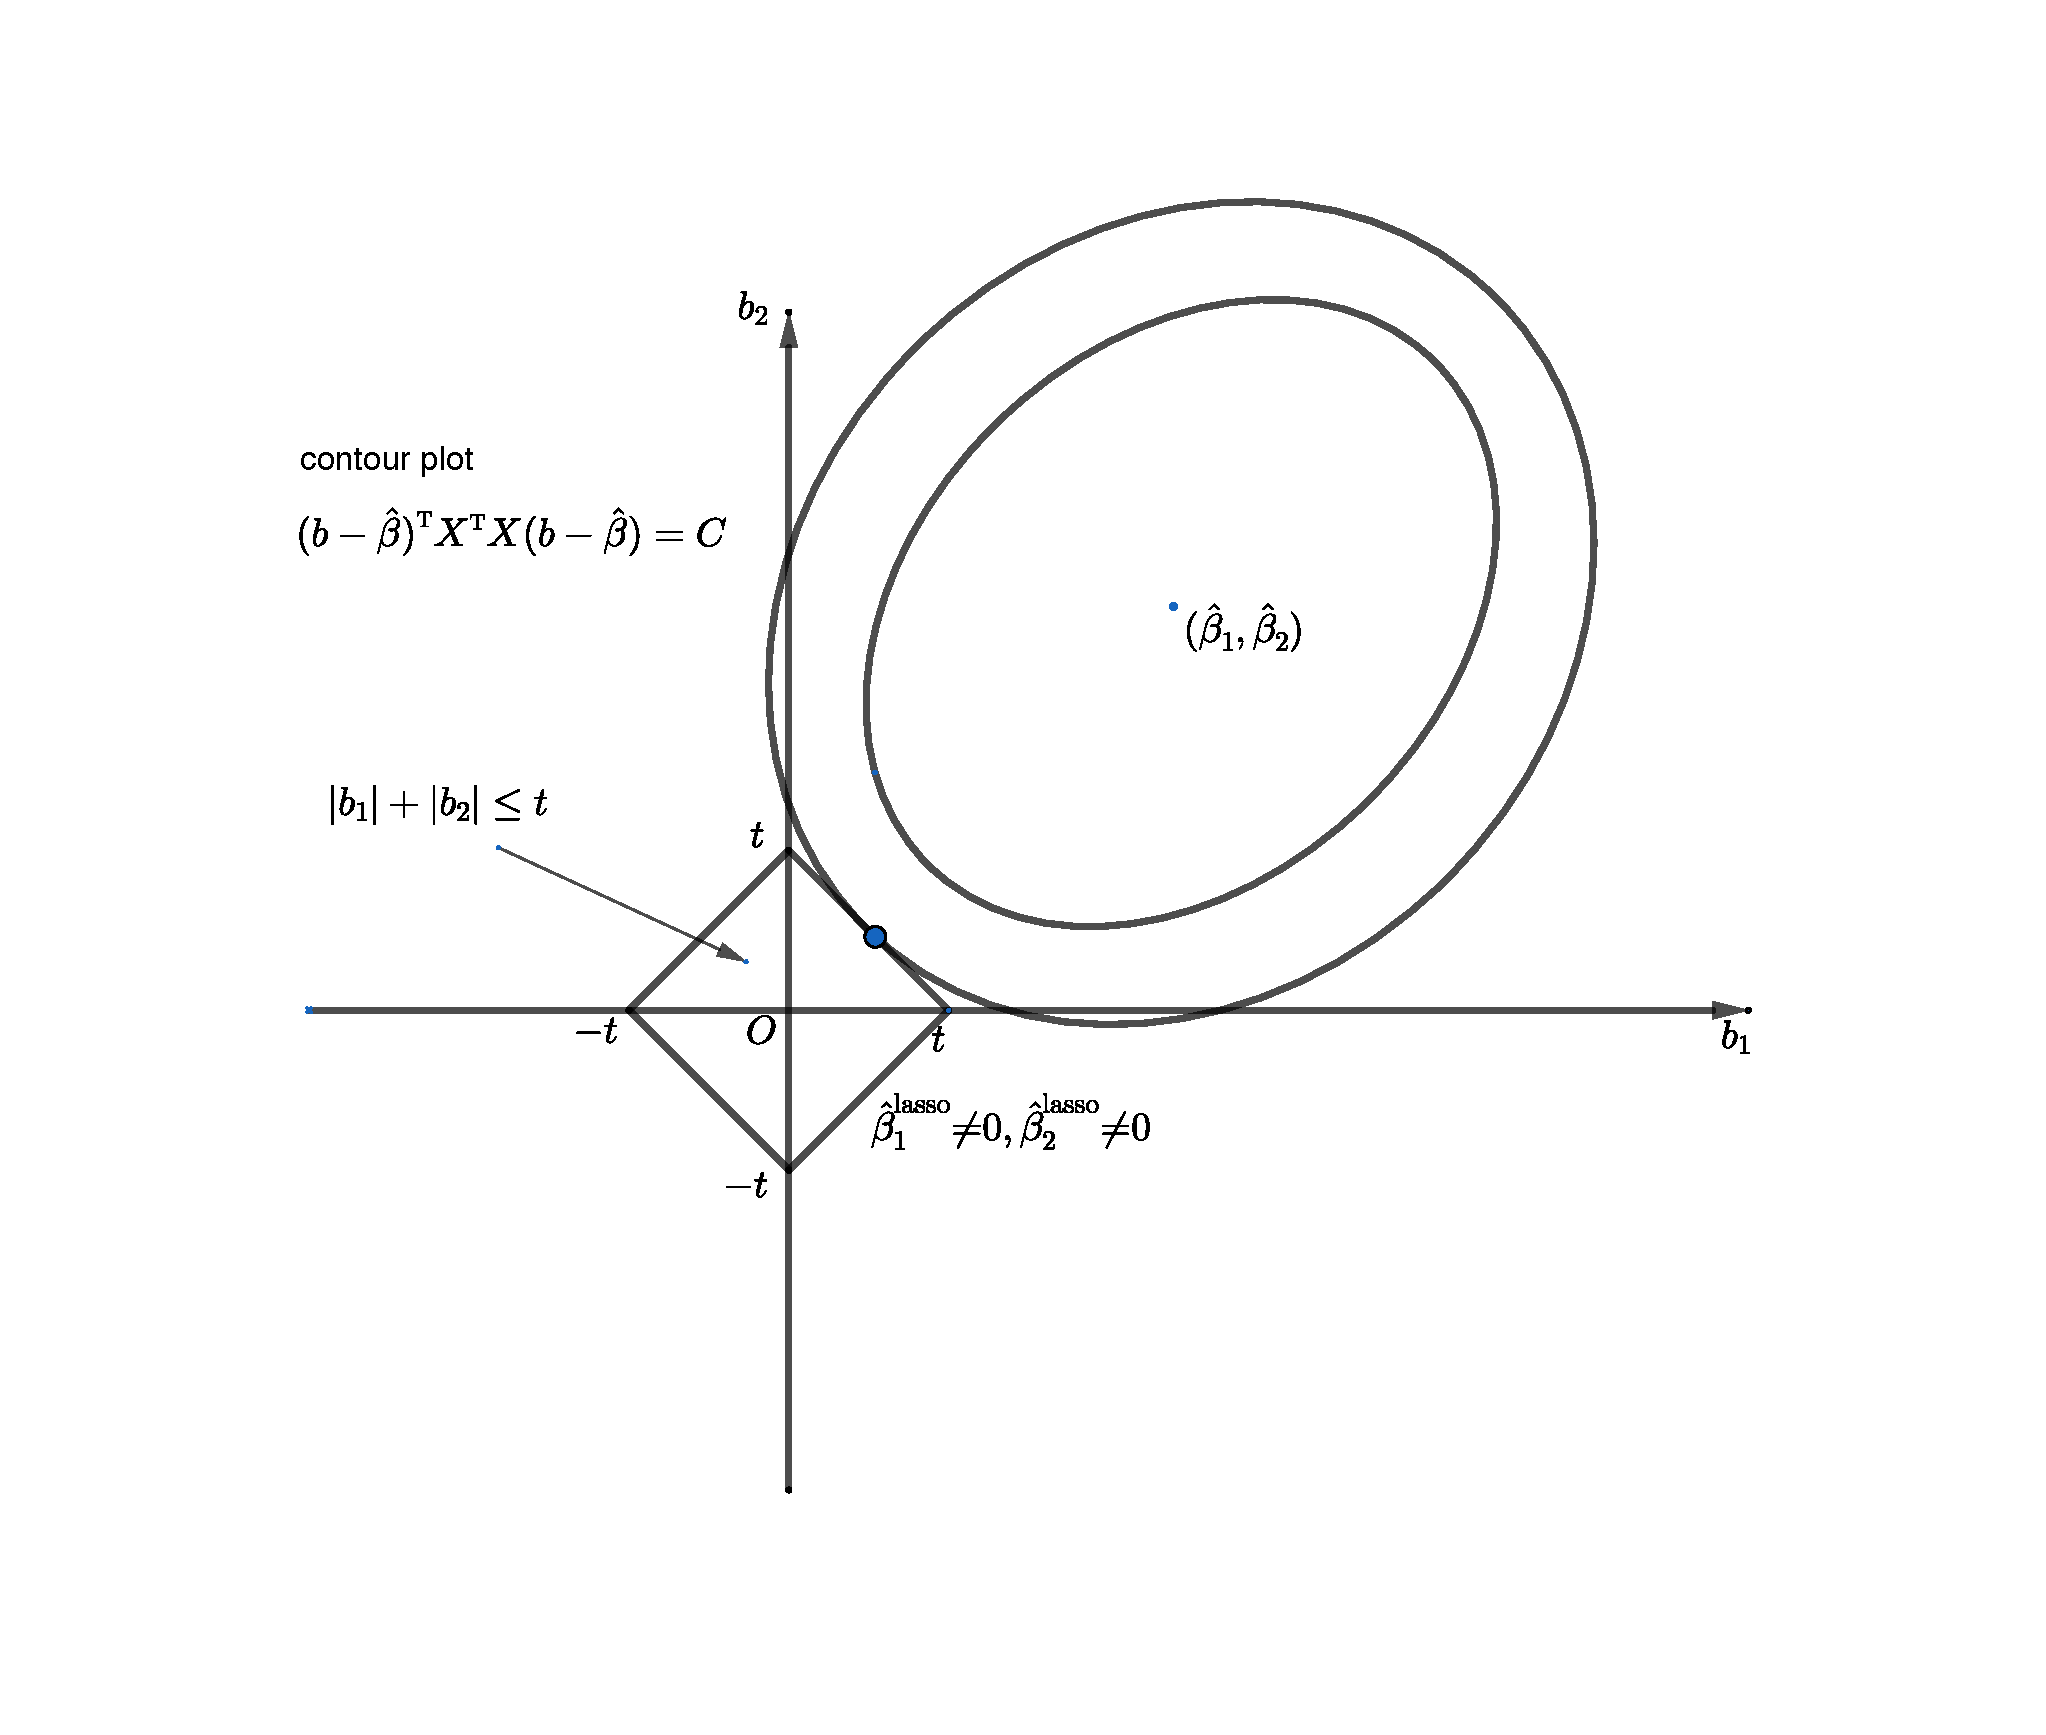
\includegraphics[width = 0.7\textwidth]{figures/lassogeometry2.pdf}
\caption{Lasso with a non-sparse solution}\label{fig::lasso-non-sparse}

\end{figure}


In contrast, the restriction region of the ridge is a circle, so the ridge solution does not hit any axis unless the original OLS coefficient is zero. Figure \ref{fig::ridge-non-sparse} shows the general ridge estimator. 

\begin{figure}
\centering 
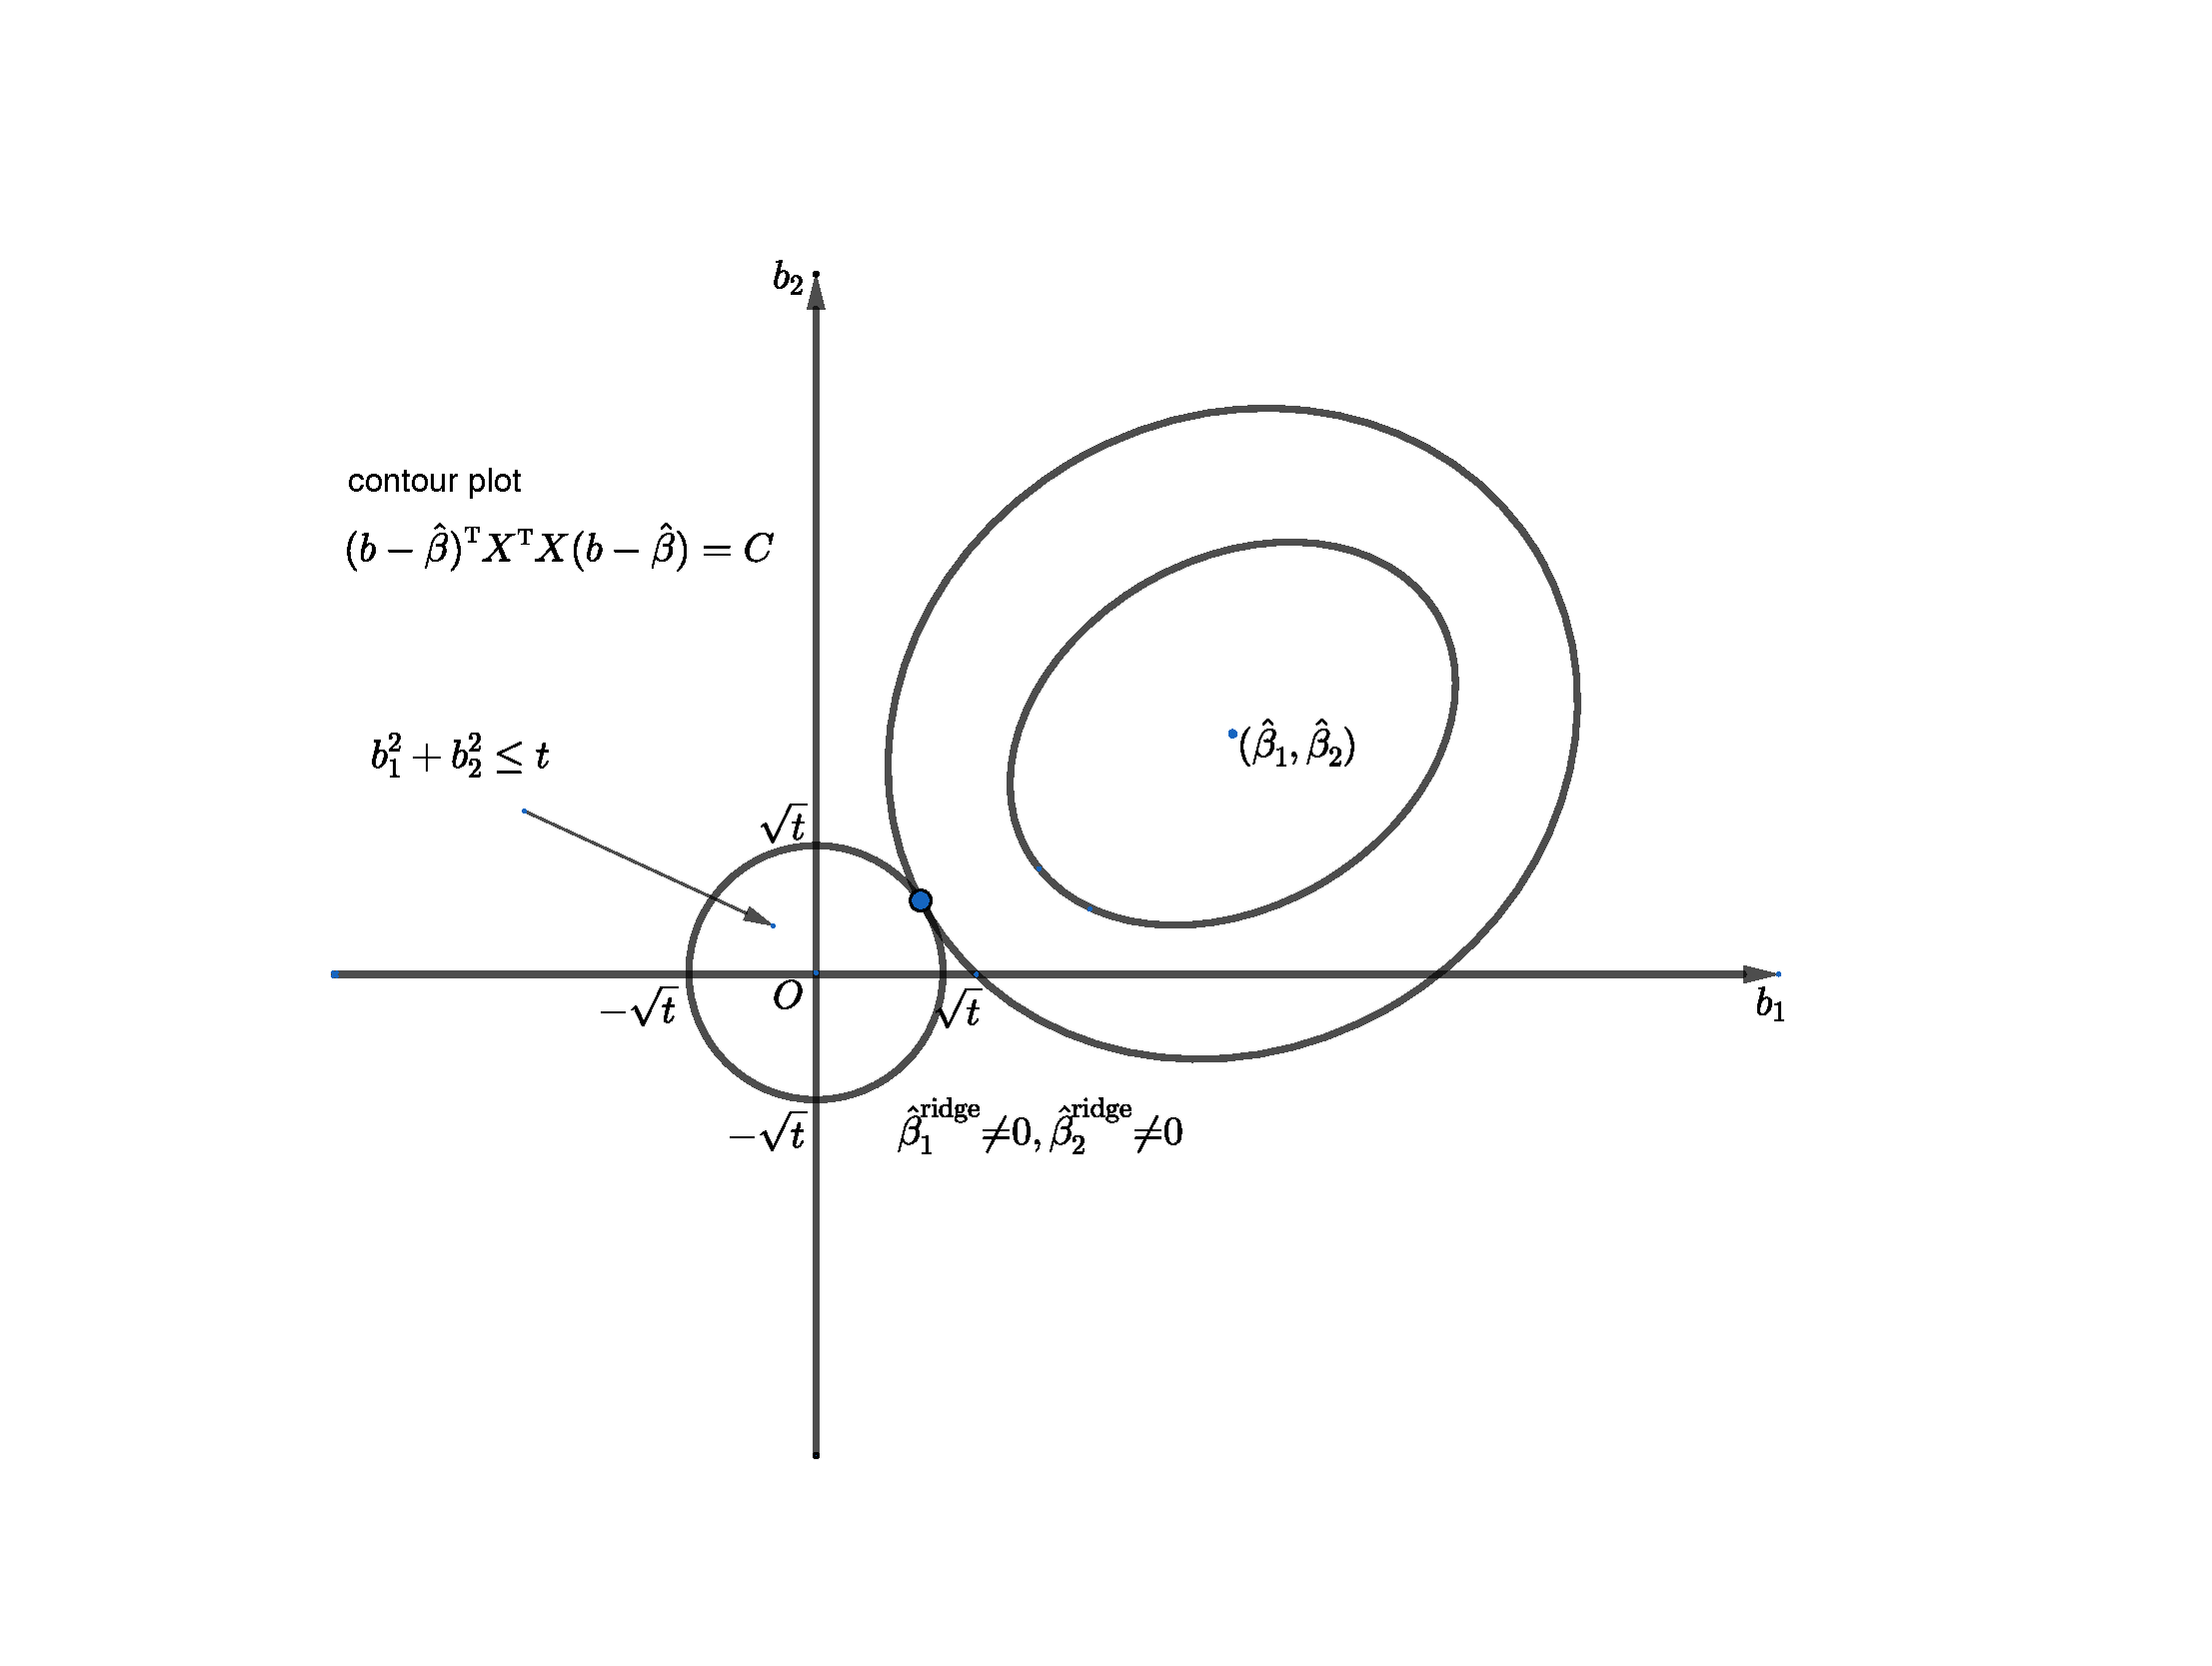
\includegraphics[width = 0.7\textwidth]{figures/ridgegeometry.pdf}
\caption{Ridge}
\label{fig::ridge-non-sparse}

\end{figure}


\section{Computing the lasso via coordinate descent}



Many efficient algorithms can solve the lasso problem. The \ri{glmnet} package in \ri{R} uses the coordinate descent algorithm based on the form \eqref{eq:lasso-form1} \citep{friedman2007pathwise, friedman2010regularization}. I will first review a lemma which is the stepstone for the algorithm. 


\subsection{The soft-thresholding lemma}


Let $\textup{sign}(x)$ denote the sign of a real number $x$, which equals $1, 0, -1$ if $x>0, x=0, x<0$, respectively. Let $(x)_{+}=\max(x,0)$
denote the positive part of a real number $x$.  

\begin{lemma}
\label{lemma:softthresholding-lemma}Given $b_{0}$ and $\lambda \geq 0$, we have 
\begin{align*}
\arg\min_{b\in \mathbb{R}}\frac{1}{2}(b-b_{0})^{2}+\lambda|b| & =\textup{sign}(b_{0})\left(|b_{0}|-\lambda\right)_{+}\\
 & =\begin{cases}
b_{0}-\lambda, & \text{if }b_{0}\geq\lambda,\\
0 & \text{if }-\lambda\leq b_{0}\leq\lambda,\\
b_{0}+\lambda & \text{if }b_{0}\leq-\lambda . 
\end{cases}
\end{align*}
\end{lemma}



The solution in Lemma \ref{lemma:softthresholding-lemma} is a function
of $b_{0}$ and $\lambda$, and we will use the notation 
\[
S(b_{0},\lambda)=\textup{sign}(b_{0})\left(|b_{0}|-\lambda\right)_{+}
\]
from now on, where $S$ denotes the soft-thresholding operator. For a given $\lambda>0$, it is a function of $b_{0}$
illustrated by Figure \ref{fig::soft-threshholding-function}. The proof of Lemma \ref{lemma:softthresholding-lemma}
is to solve the optimization problem. It is tricky since we cannot naively solve the first-order condition due to the non-smoothness of $|b|$ at $0$. Nevertheless, it is only a one-dimensional optimization problem, and I relegate the proof as Problem \ref{hw14::soft-thresholding-lemma}. 



\begin{figure}
\centering 
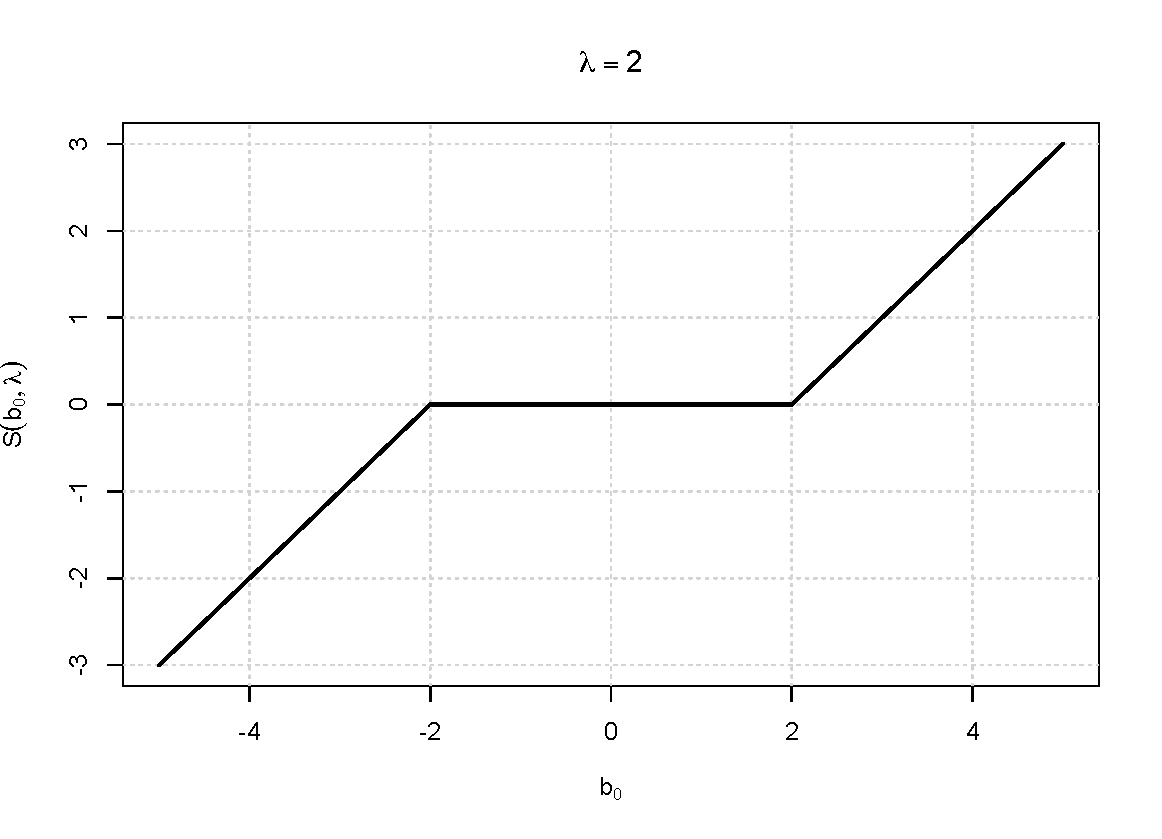
\includegraphics[scale=0.6]{figures/softthresholdingplot}

\caption{Soft-thresholding}\label{fig::soft-threshholding-function}

\end{figure}




\subsection{Coordinate descent for the lasso}

For a given $\lambda>0$, we can use the following algorithm: 
\begin{enumerate}
\item Standardize the data as Condition \ref{condition::standardization}. 
So we need to solve a lasso problem without the intercept. For simplicity
of derivation, we change the scale of the residual sum of squares
without essentially changing the problem:
\[
\min_{b_{1},\ldots,b_{p}}\frac{1}{2n}\sumn(y_{i} -b_{1}x_{i1}-\cdots-b_{p}x_{ip})^{2}+\lambda\sum_{j=1}^{p}|b_{j}|.
\]
Initialize $\hat{\beta}.$
\item Update $\hat{\beta}_{j}$ given all other coefficients. Define the
partial residual as $r_{ij}=y_{i}-\sum_{k\neq j}\hat{\beta}_{k} x_{ik}$.
Updating $\hat{\beta}_{j}$ is equivalent to minimizing
\[
\frac{1}{2n}\sumn(r_{ij}-b_{j}x_{ij})^{2}+\lambda|b_{j}|.
\]
Define 
\[
\hat{\beta}_{j,0}=\frac{\sumn x_{ij}r_{ij}}{\sumn x_{ij}^{2}}=n^{-1}\sumn x_{ij}r_{ij}
\]
as the OLS coefficient of the $r_{ij}$'s on the $x_{ij}$'s, so 
\begin{align*}
\frac{1}{2n}\sumn(r_{ij}-b_{j}x_{ij})^{2} & =\frac{1}{2n}\sumn(r_{ij}-\hat{\beta}_{j,0}x_{ij})^{2}+\frac{1}{2n}\sumn x_{ij}^{2}(b_{j}-\hat{\beta}_{j,0})^{2}\\
 & =\text{constant}+\frac{1}{2}(b_{j}-\hat{\beta}_{j,0})^{2}.
\end{align*}
Then updating $\hat{\beta}_{j}$ is equivalent to minimizing $\frac{1}{2}(b_{j}-\hat{\beta}_{j,0})^{2}+\lambda|b_{j}|$.
Lemma \ref{lemma:softthresholding-lemma} implies 
\[
\hat{\beta}_{j}=S(\hat{\beta}_{j,0},\lambda).
\]
\item Iterate until convergence. 
\end{enumerate}


Does the algorithm always converge? 
The theory of \citet{tseng2001convergence} ensures it converges, but this is beyond the scope of this book. 
We can start with a large $\lambda$ and all zero coefficients. We then
gradually decrease $\lambda$, and for each $\lambda$, we apply the
above algorithm. We finally select $\lambda$ via $K$-fold cross-validation. Since we gradually decrease $\lambda$, the initial values from the last step are very close to the minimizer and the algorithm converges fairly fast. 


\section{Example: comparing OLS, ridge and lasso}\label{sec::lasso-example}

In the Boston housing data, the OLS, ridge, and lasso have similar performance in out-of-sample prediction. Lasso and ridge have similar coefficients. See Figure \ref{fig::ridge-lasso-coefficients-boston}(a). 

\begin{lstlisting}
> library("mlbench")
> library("glmnet")
> library("MASS")
> data(BostonHousing)
> 
> ## training and testing data
> set.seed(230)
> nsample = dim(BostonHousing)[1]
> trainindex = sample(1:nsample, floor(nsample*0.9))
> 
> xmatrix = model.matrix(medv ~ ., data = BostonHousing)[, -1]
> yvector = BostonHousing$medv 
> dat = data.frame(yvector, xmatrix)
> 
> ## linear regression
> bostonlm = lm(yvector ~ ., data = dat[trainindex, ])
> predicterror = dat$yvector[- trainindex] - 
+                     predict(bostonlm, dat[- trainindex, ])
> mse.ols = sum(predicterror^2)/length(predicterror)
> 
> ## ridge regression 
> lambdas= seq(0, 5, 0.01)
> lm0 = lm.ridge(yvector ~ ., data = dat[trainindex, ],
+                lambda = lambdas)
> coefridge = coef(lm0)[which.min(lm0$GCV), ]
> predicterrorridge = dat$yvector[- trainindex] -
+   cbind(1, xmatrix[- trainindex, ])%*%coefridge
> mse.ridge = sum(predicterrorridge^2)/length(predicterrorridge)
> 
> ## lasso 
> cvboston = cv.glmnet(x = xmatrix[trainindex, ], y = yvector[trainindex])
> coeflasso = coef(cvboston, s = "lambda.min")
> predicterrorlasso = dat$yvector[- trainindex] -
+                         cbind(1, xmatrix[- trainindex, ])%*%coeflasso
> mse.lasso = sum(predicterrorlasso^2)/length(predicterrorlasso)
> 
> c(mse.ols, mse.ridge, mse.lasso)
[1] 29.37365 29.07174 28.88161
\end{lstlisting}

\begin{figure}[ht]
\centering
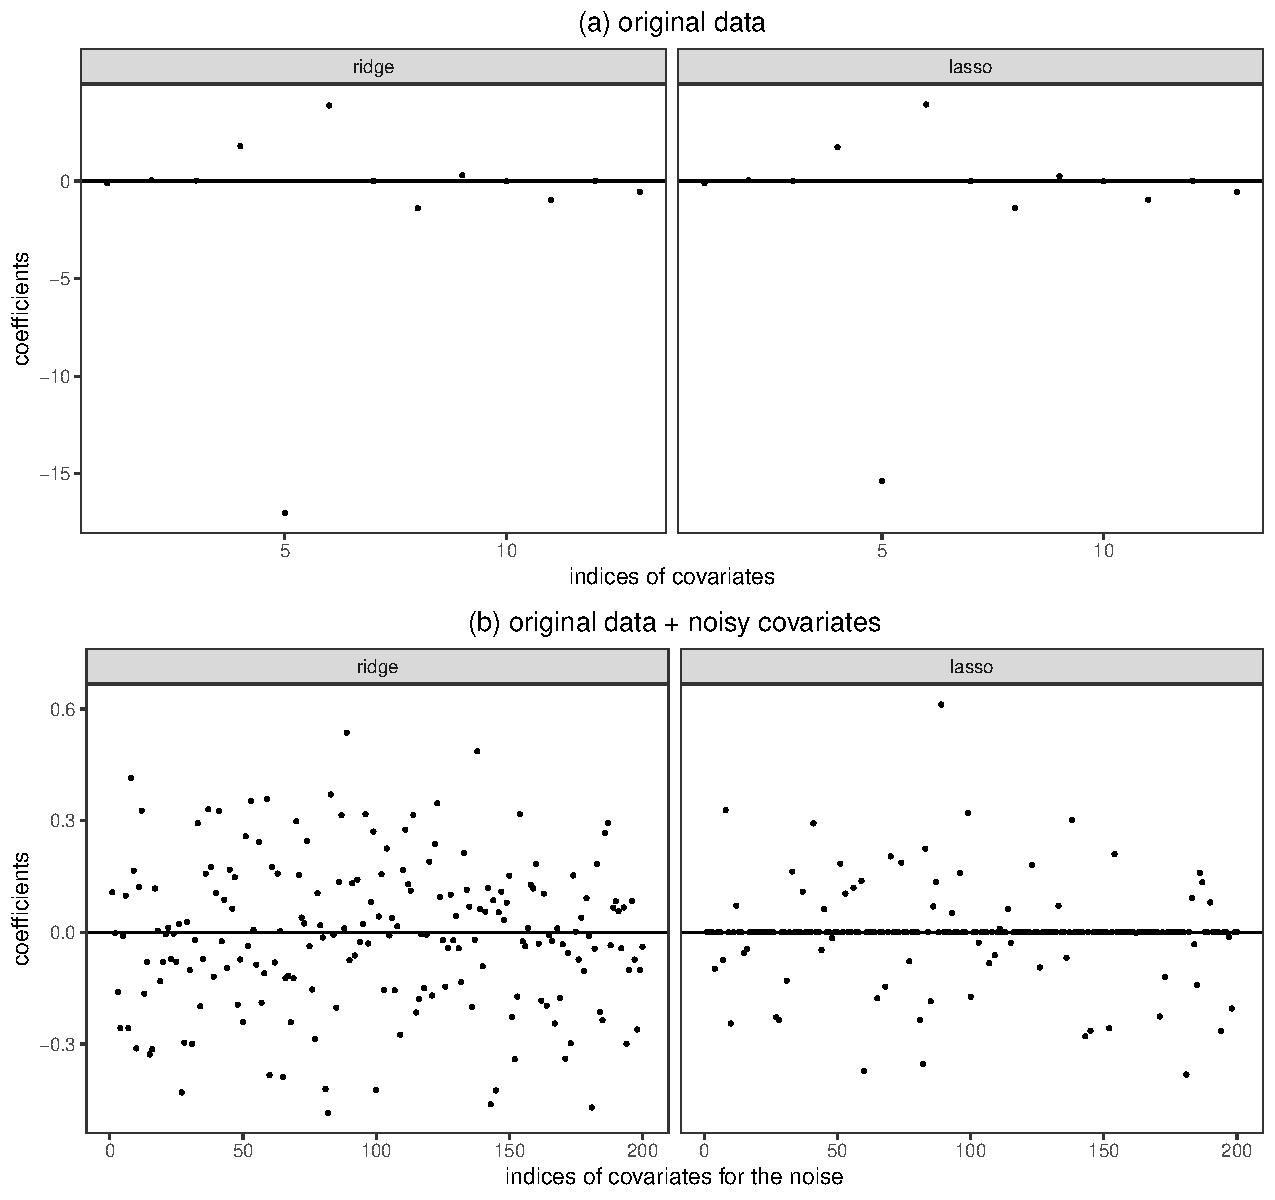
\includegraphics[width = \textwidth]{figures/ridge_lasso_coef_bostonhousing.pdf}
\caption{Comparing ridge and lasso}
\label{fig::ridge-lasso-coefficients-boston}
\end{figure}



But if we artificially add 200 columns of covariates of pure noise $\N(0,1)$, then the ridge and lasso perform much better. Lasso can automatically shrink many coefficients to zero. See   Figure \ref{fig::ridge-lasso-coefficients-boston}(b). 

\begin{lstlisting}
> ## adding more noisy covariates
> n.noise = 200
> xnoise  = matrix(rnorm(nsample*n.noise), nsample, n.noise)
> xmatrix = cbind(xmatrix, xnoise)
> dat = data.frame(yvector, xmatrix)
> 
> ## linear regression
> bostonlm = lm(yvector ~ ., data = dat[trainindex, ])
> predicterror = dat$yvector[- trainindex] - 
+   predict(bostonlm, dat[- trainindex, ])
> mse.ols = sum(predicterror^2)/length(predicterror)
> 
> ## ridge regression 
> lambdas= seq(100, 150, 0.01)
> lm0 = lm.ridge(yvector ~ ., data = dat[trainindex, ],
+                lambda = lambdas)
> coefridge = coef(lm0)[which.min(lm0$GCV), ]
> predicterrorridge = dat$yvector[- trainindex] -
+   cbind(1, xmatrix[- trainindex, ])%*%coefridge
> mse.ridge = sum(predicterrorridge^2)/length(predicterrorridge)
> 
> 
> ## lasso 
> cvboston = cv.glmnet(x = xmatrix[trainindex, ], y = yvector[trainindex])
> coeflasso = coef(cvboston, s = "lambda.min")
> 
> predicterrorlasso = dat$yvector[- trainindex] -
+   cbind(1, xmatrix[- trainindex, ])%*%coeflasso
> mse.lasso = sum(predicterrorlasso^2)/length(predicterrorlasso)
> 
> c(mse.ols, mse.ridge, mse.lasso)
[1] 41.80376 33.33372 32.64287
\end{lstlisting}



 
 

\section{Other shrinkage estimators}

A general class of shrinkage estimators is the bridge estimator \citep{frank1993statistical}: 
\[
\hat{\beta}(\lambda)=\arg\min_{b_{0},b_{1},\ldots,b_{p}}\left\{ \textsc{rss}(b_0,b_1,\ldots,b_p) +\lambda\sum_{j=1}^{p}|b_{j}|^{q}\right\} 
\]
or, by duality, 
\begin{align*}
\hat{\beta}(t) & =\arg\min_{b_{0},b_{1},\ldots,b_{p}} \textsc{rss}(b_0,b_1,\ldots,b_p)  \\
 & \ \text{s.t. }\sum_{j=1}^{p}|b_{j}|^{q}\ensuremath{\leq t.}
\end{align*}
Figure \ref{fig::general-shrinkage-estimators} shows the constraints corresponding to different values of $q$. 





\citet{zou2005regularization} proposed the elastic net which combines the penalties of the lasso and ridge: 
\[
\hat{\beta}^{\text{enet}}(\lambda,\alpha)=\arg\min_{b_{0},b_{1},\ldots,b_{p}}\left[ \textsc{rss}(b_0,b_1,\ldots,b_p)  +\lambda\sum_{j=1}^{p}\left\{ \alpha b_{j}^{2}+(1-\alpha)|b_{j}|\right\} \right].
\]
Figure \ref{fig::elasticnet-penalty} compares the constraints corresponding to the ridge, lasso, and elastic net. Because the constraint of the elastic net is not smooth, it encourages sparse solutions in the same way as the lasso. Due to the ridge penalty, the elastic net can deal with the collinearity of the covariates better than the lasso. 


\begin{figure}
\centering 
\subfloat[$0<q<1$]{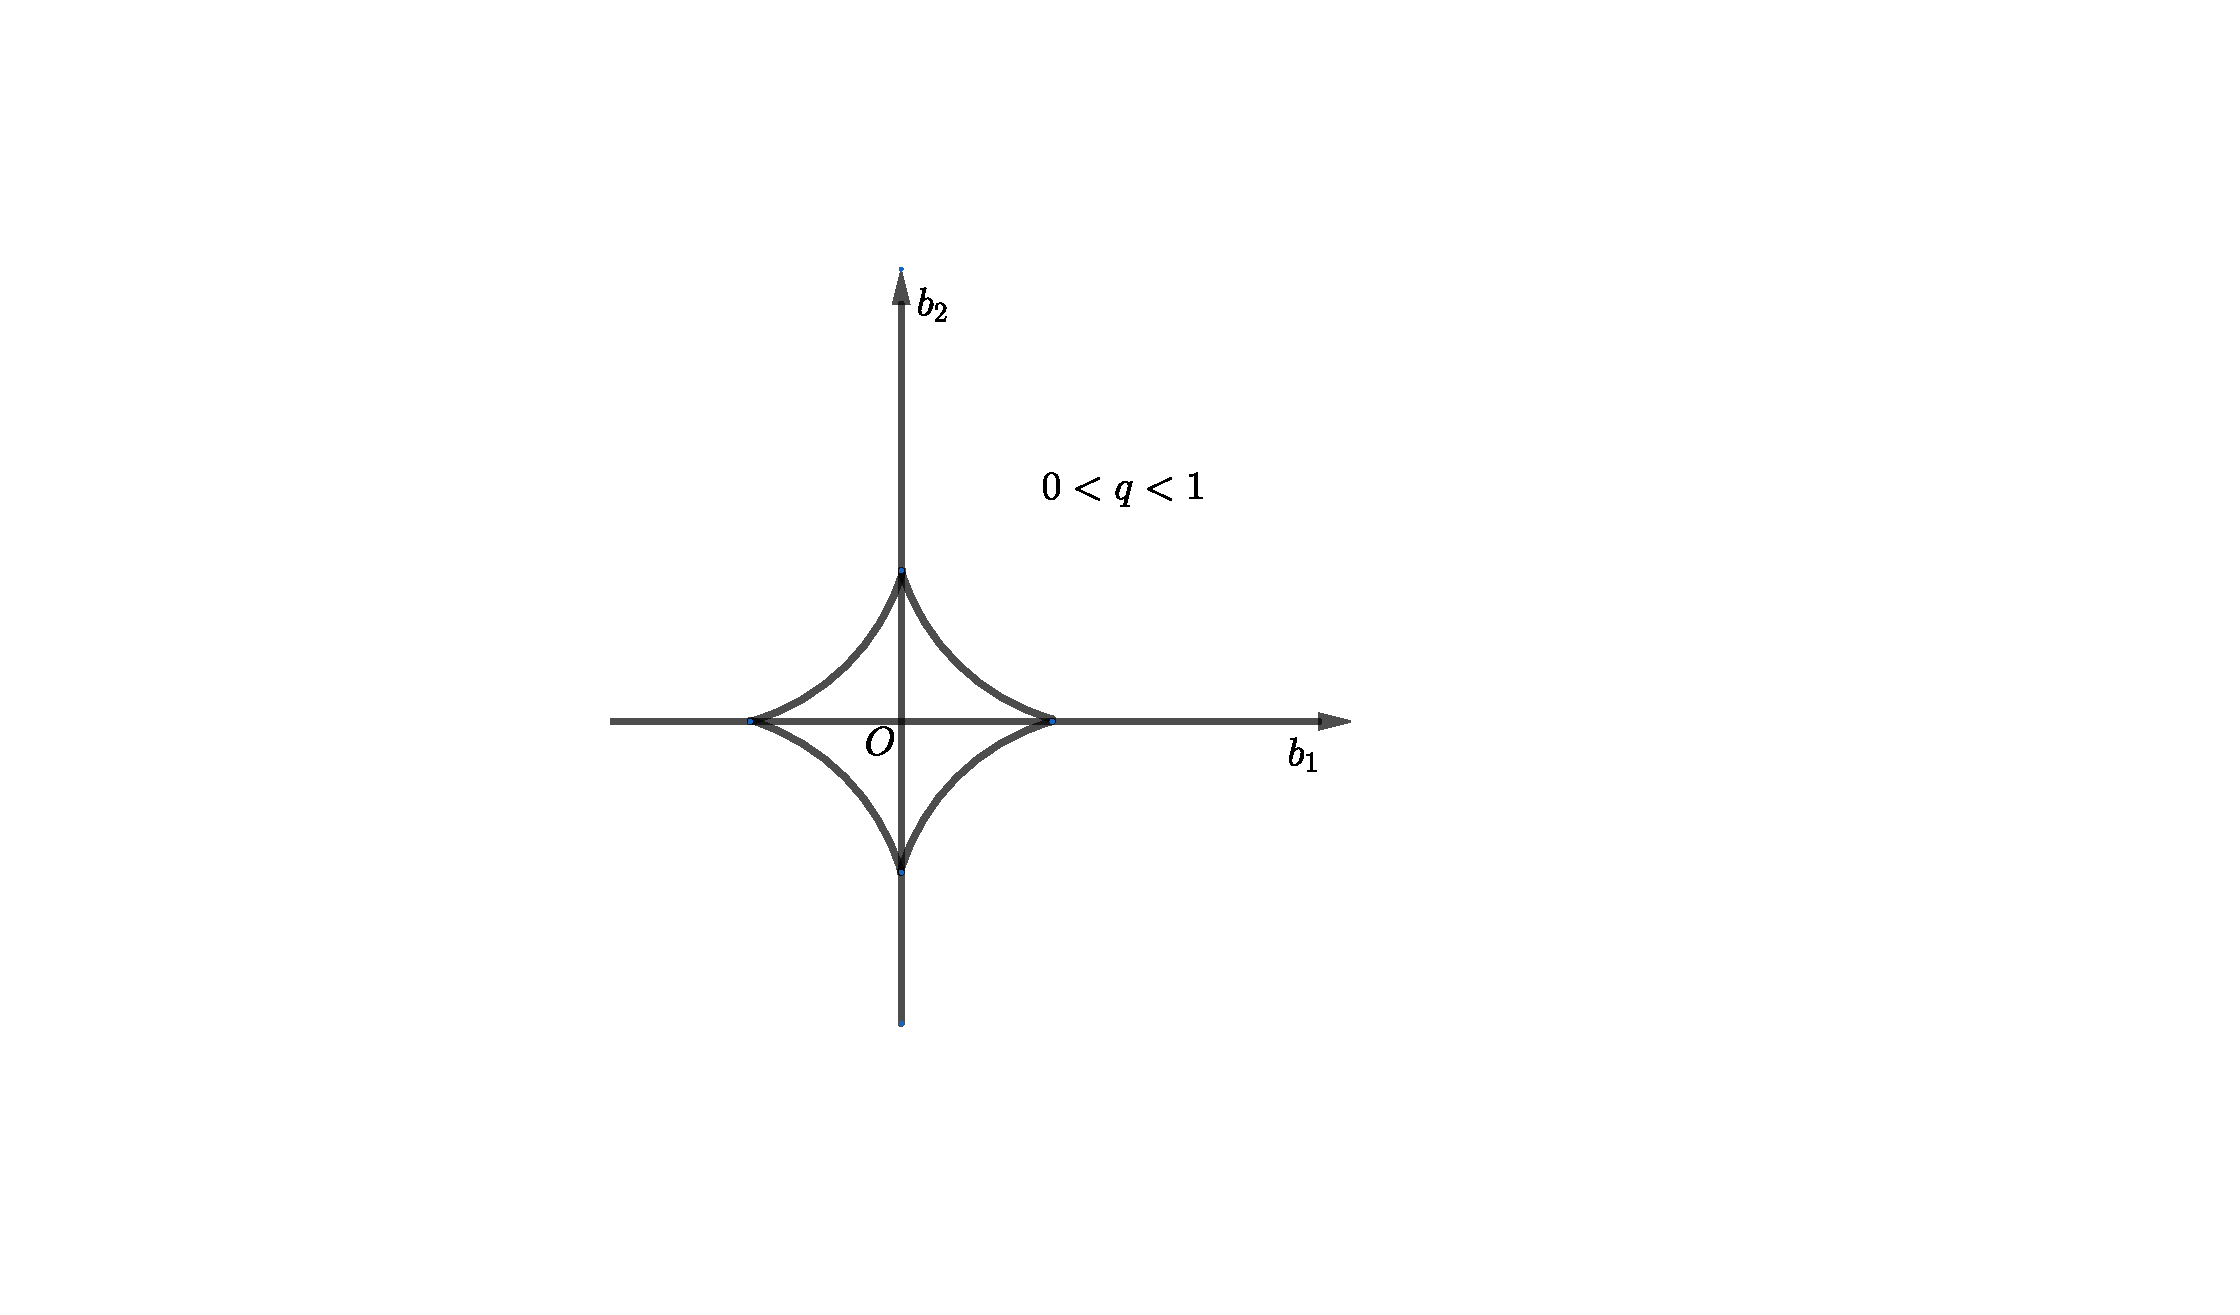
\includegraphics[width=0.33\textwidth]{figures/lq01}
}
\subfloat[$q=1$]{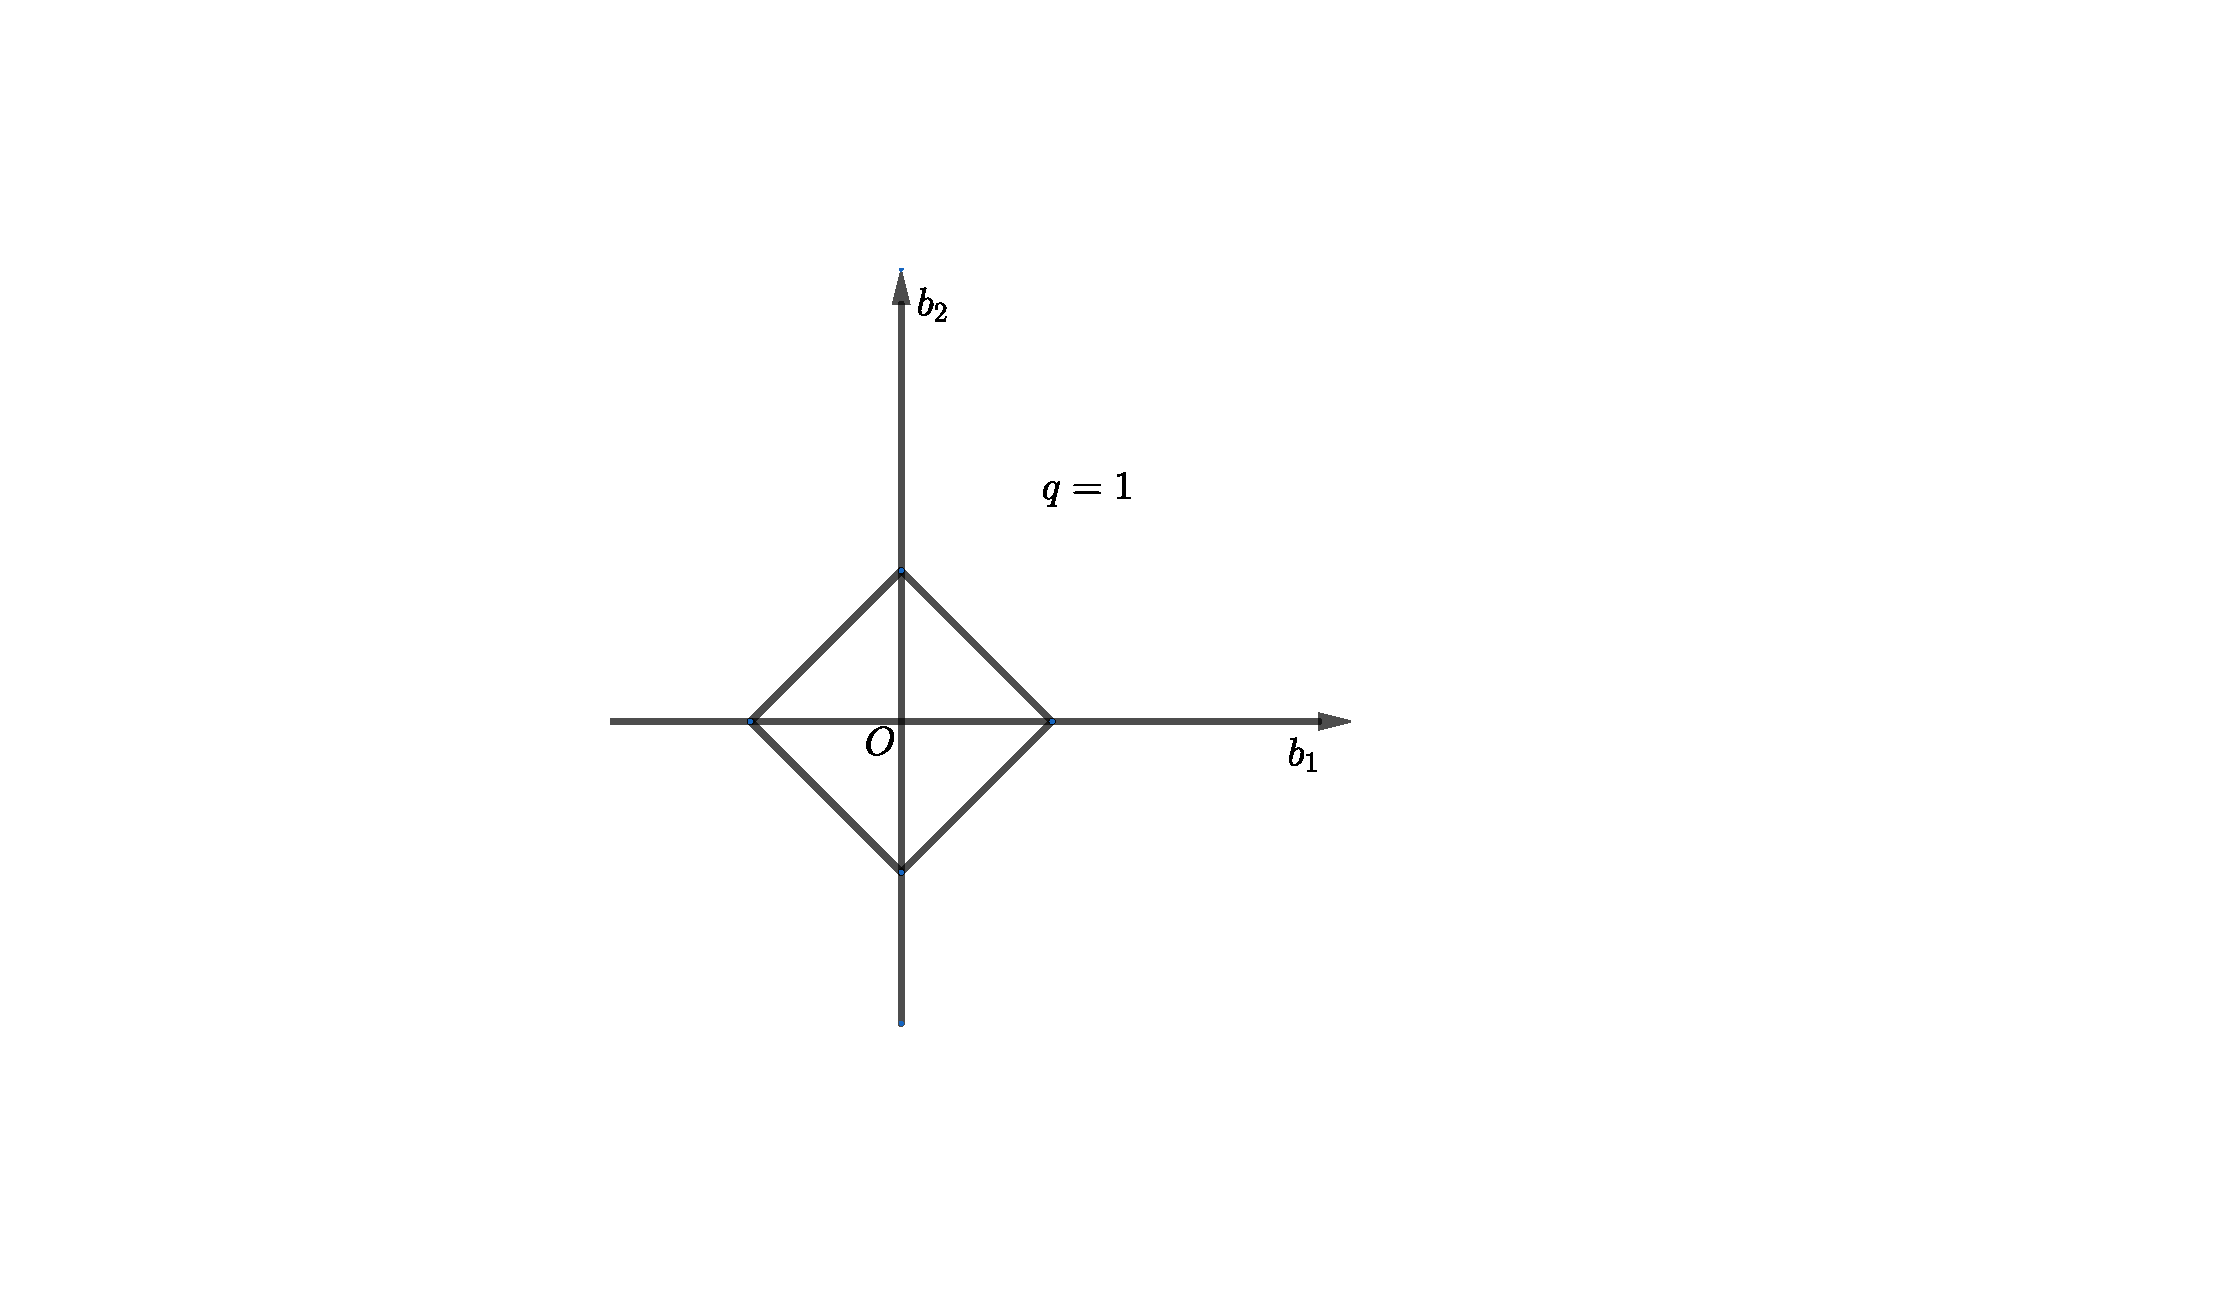
\includegraphics[width=0.33\textwidth]{figures/lq1}
}\subfloat[$q=2$]{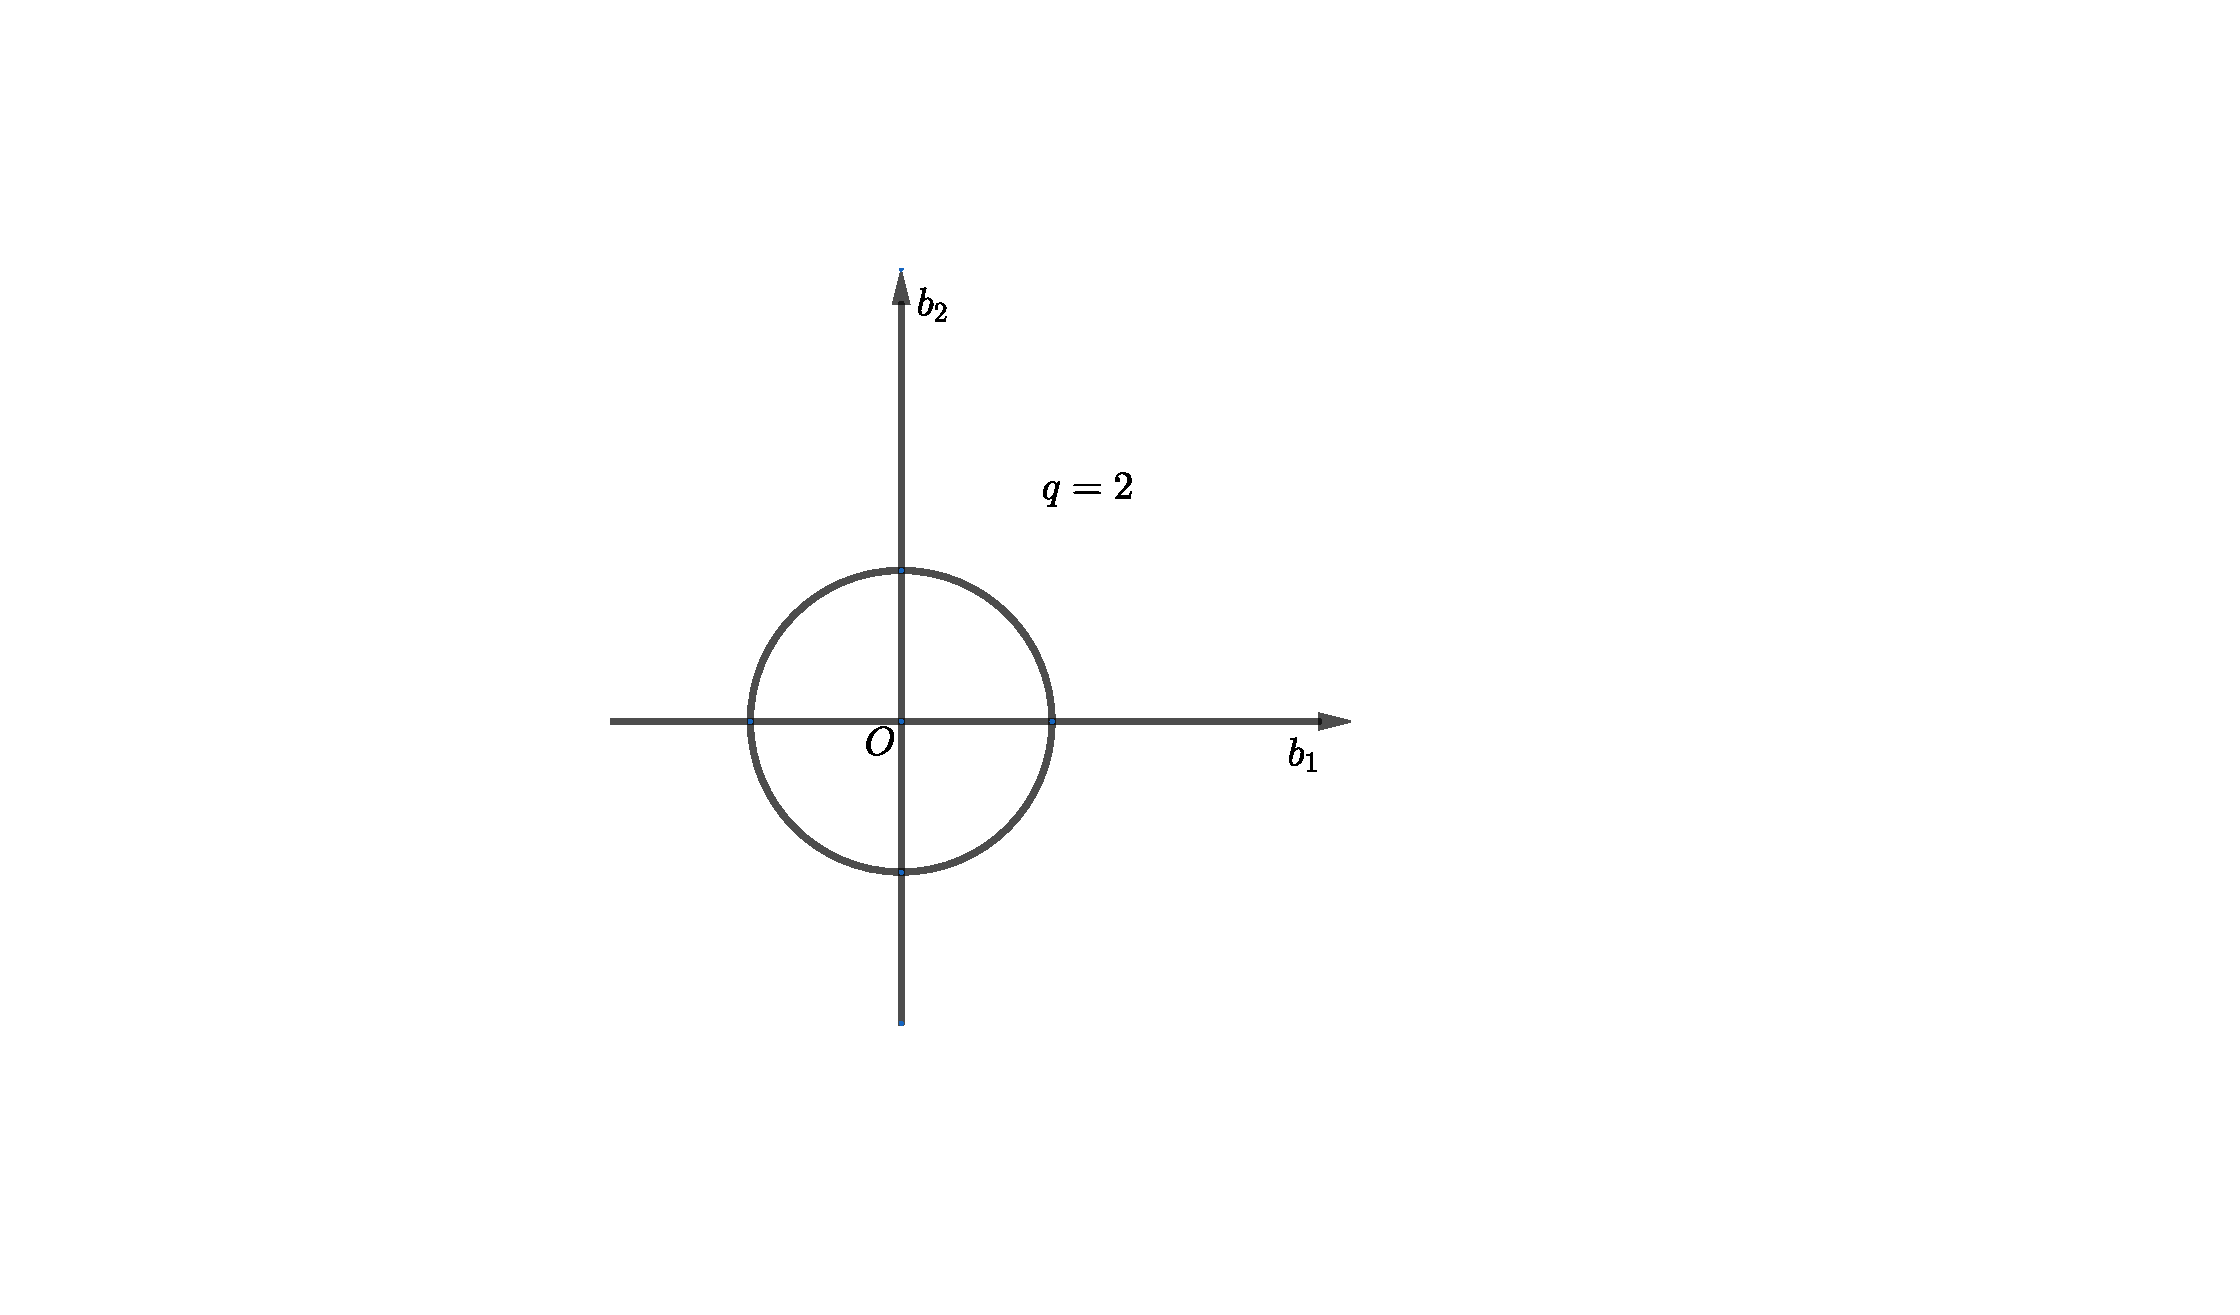
\includegraphics[width=0.33\textwidth]{figures/lq2}
}\caption{Shrinkage estimators}\label{fig::general-shrinkage-estimators}
\end{figure}




\begin{figure}
\centering
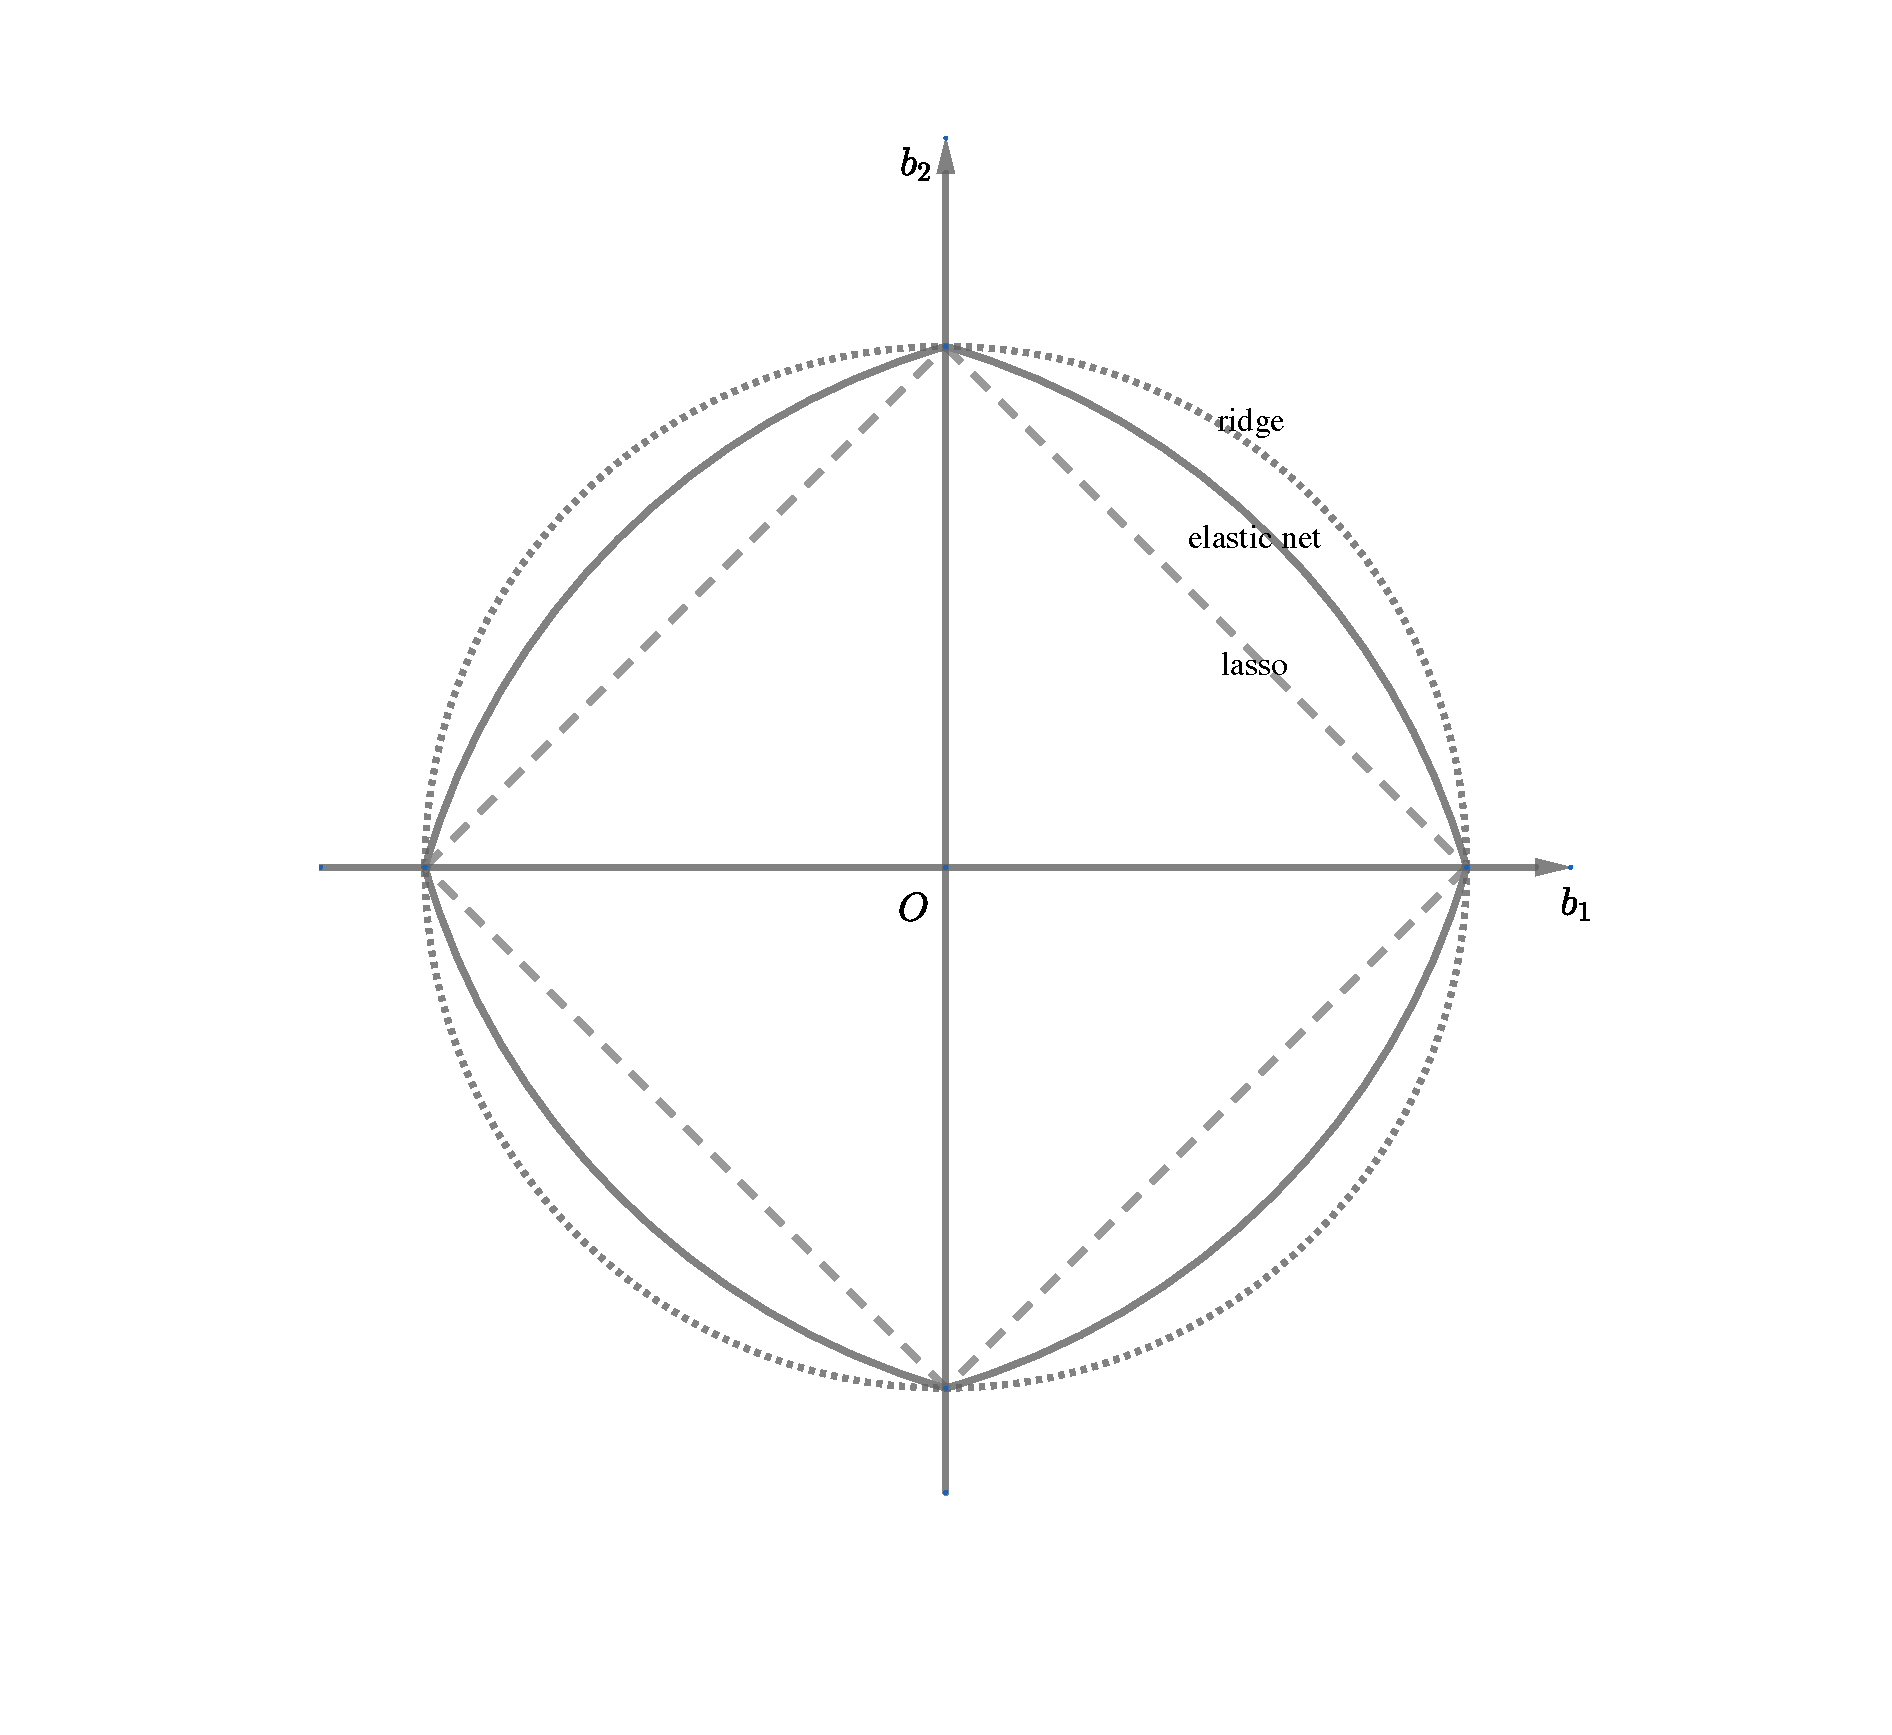
\includegraphics[width = 0.6\textwidth]{figures/elasticnetpenalty.pdf}
\caption{Comparing the ridge, lasso, and elastic net}
\label{fig::elasticnet-penalty}
\end{figure}



\citet{friedman2007pathwise} proposed to use the coordinate descent algorithm to solve for the elastic net estimator, and \citet{friedman2009glmnet} implemented it in an \ri{R} package called \ri{glmnet}. 

 
 
 
\section{Homework problems}


\paragraph{Uniqueness of the lasso prediction}\label{hw14::uniqueness-lasso-pred}


Consider the lasso problem: 
$$
\min_{b\in\mathbb{R}^{p}}   \|Y-Xb\|^{2}+\lambda\|b\|_{1} . 
$$
Show that if $\hat{\beta}^{(1)}$ and $\hat{\beta}^{(2)}$ are two solutions, then $ \alpha  \hat{\beta}^{(1)} + (1-\alpha)  \hat{\beta}^{(2)}$ is also a solution for any $0\leq  \alpha  \leq 1$. Show that $X \hat{\beta}^{(1)} = X\hat{\beta}^{(2)}$ must hold. 


Hint: The function $\| \cdot \|^2$ is strongly convex. That is, for any $v_1, v_2$ and $ 0< \alpha < 1$, we have
$$
\|   \alpha  v_1  +(1-\alpha ) v_2     \|^2 \leq \alpha \| v_1 \|^2 + (1- \alpha ) \| v_2 \|^2
$$
and the inequality holds when $v_1 \neq v_2$.  The function $\|\cdot \|$ is convex. That is, for any $v_1, v_2$ and $ 0< \alpha < 1$, we have
$$
\|   \alpha  v_1  +(1-\alpha ) v_2     \|_1 \leq \alpha \| v_1 \|_1 + (1- \alpha ) \| v_2 \|_1.
$$

\paragraph{The soft-thresholding lemma}\label{hw14::soft-thresholding-lemma}

Prove Lemma \ref{lemma:softthresholding-lemma}. 

\paragraph{Penalized OLS with an orthogonal design matrix}\label{hw14::orthogonal-ols-pen}

Consider the special case with standardized and orthogonal design
matrix:
\[
X^{\T}1_{n}=0,\qquad X^{\T}X=I_{p}.
\]
For a fixed $\lambda\geq0$, find the explicit formulas of the $j$th coordinates of the following
estimators in terms of the corresponding $j$th coordinate of the OLS estimator $\hat{\beta}_j$ and
$\lambda$ $(j=1,\ldots, p)$:
\begin{align*}
\hat{\beta}^{\text{ridge}}(\lambda) & =\arg\min_{b\in\mathbb{R}^{p}}\left\{ \|Y-Xb\|^{2}+\lambda\|b\|^{2}\right\} ,\\
\hat{\beta}^{\text{lasso}}(\lambda) & =\arg\min_{b\in\mathbb{R}^{p}}\left\{ \|Y-Xb\|^{2}+\lambda\|b\|_{1}\right\} ,\\
\hat{\beta}^{\text{enet}}(\lambda) & =\arg\min_{b\in\mathbb{R}^{p}}\left\{ \|Y-Xb\|^{2}+\lambda  (  \alpha \|b\|^{2} + (1-\alpha) \|b\|_{1} )  \right\}  ,\\
\hat{\beta}^{\text{subset}}(\lambda) & =\arg\min_{b\in\mathbb{R}^{p}}\left\{ \|Y-Xb\|^{2}+\lambda\|b\|_{0}\right\} ,
\end{align*}
where 
\[
 \|b\|^2 =  \sum_{j=1}^{p}b_{j}^{2},\quad\|b\|_{1}=\sum_{j=1}^{p}|b_{j}|,\quad\|b\|_{0}=\sum_{j=1}^{p}1(b_{j}\neq0).
\]


\paragraph{Standardization in the elastic net}\label{hw14::standardization-enet}


For fixed $\lambda$ and $\alpha$, show that the intercept in 
$
\hat{\beta}^{\text{enet}}(\lambda,\alpha)
$
equals zero under the standardization in Condition \ref{condition::standardization}. 


\paragraph{Coordinate descent for the elastic net}\label{hw14::enet-coordinate-descent}

Give the detailed coordinate descent algorithm for the elastic net. 


\paragraph{Reducing elastic net to lasso}\label{hw14::enet-lasso}


Consider the following form of the elastic net:
$$
\arg\min_{ b \in\mathbb{R}^{p}}  \|  Y -Xb \|^2 + \lambda  \{  \alpha \| b\|^2 + (1-\alpha) \| b \|_1 \} .
$$
Show that it reduces to the following lasso:
$$
\arg\min_{b\in\mathbb{R}^{p}}  \|  \tilde Y -  \tilde Xb \|^2 + \tilde  \lambda  \| b \|_1,
$$
where 
$$
\tilde Y = \begin{pmatrix}
Y \\
0_p
\end{pmatrix},\quad
\tilde X = \begin{pmatrix}
X \\
\sqrt{\lambda \alpha} I_p
\end{pmatrix},\quad
\tilde{\lambda} = \lambda  (1-\alpha).
$$

Hint: Use the result in Problem \ref{hw13::ridge-data-aug}.




\paragraph{Reducing lasso to iterative ridge}\label{hw14::lasso-iterative-ridge} 



Based on the simple result 
$$
\min_{ac=b} (a^2+c^2)/2 = |b|,
$$
for scalars $a,b,c$, \citet{hoff2017lasso} rewrote the lasso problem 
$$
\min_{b\in  \mathbb{R}^p } \{   \| Y-Xb\|^2 + \lambda \|b\|_1 \}
$$
as
$$
\min_{u,v\in  \mathbb{R}^p } \{   \| Y-X(u\circ v)\|^2 + \lambda ( \|u\|^2 + \|v\|^2 )/2 \}
$$
where $\circ$ denotes the component-wise product of vectors. \citet[][Lemma 1]{hoff2017lasso} showed that a local minimum of the new problem must be a local minimum of the lasso problem. 

Show that the new problem can be solved based on the following iterative ridge regressions:
\begin{enumerate}
\item
given $u$, we update $v$ based on the ridge regression of $Y$ on $X_u$ with tuning parameter $\lambda /2$, where $X_u = X \text{diag}(u_1,\ldots, u_p)$;
\item
given $v$, we update $u$ based on the ridge regression of $Y$ on $X_v$ with tuning parameter $\lambda/2$, where $X_v = X \text{diag}(v_1,\ldots, v_p)$.

\end{enumerate}


 

\paragraph{More noise in the Boston housing data}

The Boston housing data have $n=506$ observations. Add $p=n$ columns of covariates of random noise, and compare OLS, ridge, and lasso, as in Section \ref{sec::lasso-example}. Add $p=2n$ columns of covariates of random noise, and compare OLS, ridge, and lasso. 

 
\paragraph{Recommended reading}


\citet{tibshirani2011regression}  gives a review of the lasso, as well as its history and recent developments. Two discussants, Professors Peter B\"uhlmann and Chris Holmes, make some excellent comments. 

 
 
